\documentclass[9pt,twocolumn,twoside]{pnas-new}
% Use the lineno option to display guide line numbers if required.

\templatetype{pnasresearcharticle} % Choose template
% {pnasresearcharticle} = Template for a two-column research article
% {pnasmathematics} %= Template for a one-column mathematics article
% {pnasinvited} %= Template for a PNAS invited submission

\usepackage{natbib}
\begin{document}


\title{Microbial symbionts buffer hosts from the consequences of environmental stochasticity}

% Use letters for affiliations, numbers to show equal authorship (if applicable) and to indicate the corresponding author
\author[a,b,1]{Joshua C. Fowler}
\author[c]{Shaun M. Ziegler}
\author[c]{Kenneth D. Whitney}
\author[c]{Jennifer A. Rudgers}
\author[a]{Tom E.X. Miller}

\affil[a]{Department of BioSciences, Rice University, Houston, TX, 77005}
\affil[b]{Department of Biology, University of Miami, Miami, FL, 33146}
\affil[c]{Department of Biology, University of New Mexico, Albuquerque, NM, 87131}

% Please give the surname of the lead author for the running footer
\leadauthor{Fowler}

% Please add a significance statement to explain the relevance of your work
\significancestatement{
	\textbf{limit = 120 out of 120 words}
    Many symbiotic microbes benefit hosts under environmental stress, which is become more frequent in an increasingly variable climate.
    Using long-term field experiments with a plant-fungal endophyte model system, we show that, by limiting host exposure to environmental extremes, microbial symbionts reduce their hosts' demographic variance.
    Because such variance has negative fitness consequences, our results identify variance buffering a novel pathway of host-symbiont mutualism.
    Species with faster life histories were more strongly buffered by symbiosis, suggesting that microbial symbionts can compensate for the lack of intrinsic tolerance of variability conferred by ``slow'' life history traits.
    Simulations revealed that increasing stochasiticity intensifies the benefits of variance buffering, suggesting a key role of microbial symbionts in promoting host resilience to climate change.
}

% Please include corresponding author, author contribution and author declaration information
\authorcontributions{
	J.C.F. contributed to data collection, data analysis, and led manuscript drafting.
	S.Z. contributed to data collection and manuscript revisions.
	K.D.W. contributed to research conception, data collection, and manuscript revisions.
	J.A.R. established transplant plots, contributed to research conception, data collection, and manuscript revisions.
	T.E.X.M. contributed to research conception, data collection, data analysis, and manuscript revisions.}
\authordeclaration{The authors declare no conflict of interest}

\correspondingauthor{\textsuperscript{1}To whom correspondence should be addressed. E-mail: jcf221\@miami.edu}

% At least three keywords are required at submission. Please provide three to five keywords, separated by the pipe symbol.
\keywords{stochasticity $|$ microbial symbiosis $|$ demography $|$ mutualism}



\begin{abstract}
	\textbf{limit = 188 out of 250 words}
	Species' persistence in increasingly variable future climates will depend on endurance of the detrimental effects of environmental stochasticity.
	Most organisms host microbiota that shield against stressful environmental conditions, but pinpointing microbial symbioses as buffers against the fitness costs of stochasticity requires experiments covering long-term variability. 
	Here, we use stochastic demographic models for seven plant species parameterized with a 14-year symbiont-removal experiment to demonstrate that microbial symbionts elevate host fitness by dampening year-to-year fluctuations in demographic performance.
	We show that \emph{Epichloë} fungal endophytes reduce variance in the fitness of their grass hosts by greater than 10\% on average across species and that reductions of up to 50\% occur for some hosts.
	Hosts with "fast" life histories that lack longevity as an intrinsic buffer experienced the greatest benefits. 
	Contributions to fitness from variance buffering were modest compared to symbiont benefits to mean fitness under the contemporary climate regime.
	Simulations of increased environmental stochasticity amplified the value of variance buffering, which surpassed symbionts' mean effects that have dominated most prior research.
	These results establish microbial-mediated variance buffering as an important yet cryptic mechanism of resilience to increasing stochasticity under global change.
\end{abstract}



\dates{This manuscript was compiled on \today}
\doi{\url{www.pnas.org/cgi/doi/10.1073/pnas.XXXXXXXXXX}}


\maketitle
\thispagestyle{firststyle}
\ifthenelse{\boolean{shortarticle}}{\ifthenelse{\boolean{singlecolumn}}{\abscontentformatted}{\abscontent}}{}




\firstpage[7]{4}
% Use \firstpage to indicate which paragraph and line will start the second page and subsequent formatting. In this example, there are a total of 11 paragraphs on the first page, counting the first level heading as a paragraph. The value {12} represents the number of the paragraph starting the second page. If a paragraph runs over onto the second page, include a bracket with the paragraph line number starting the second page, followed by the paragraph number in curly brackets, e.g. "\firstpage[4]{11}".


% If your first paragraph (i.e. with the \dropcap) contains a list environment (quote, quotation, theorem, definition, enumerate, itemize...), the line after the list may have some extra indentation. If this is the case, add \parshape=0 to the end of the list environment.
\dropcap{G}lobal climate change involves increases in environmental variability, including changes to precipitation patterns and the frequency of extreme weather events \cite{seneviratne2012changes, ipcc_2021}.
Yet, the ecological consequences of increased variability are less well understood than those of changing climate means, such as long-term warming or drying. 
Incorporating environmental variability into forecasts of population dynamics can improve predictions of the future.
Classic theory predicts that long-term population growth rates (equivalently, population mean fitness) will decline under increased environmental variability because the costs of bad years outweigh the benefits of good years -- a consequence of nonlinear averaging \cite{lewontin_population_1969,tuljapurkar_population_1982}.
For example, in unstructured populations, the long-term stochastic growth rate in a fluctuating environment ($\lambda_s$) will always be lower than the average growth rate ($\overline{\lambda}$) by an amount proportional to the environmental variance ($\sigma^2$): 
\begin{equation}
	log(\lambda_s)  \approx log(\overline{\lambda}) - \frac{\sigma^2}{2\overline{\lambda}^2}
\end{equation}

\noindent Populations structured by size or stage similarly experience costs of variability \cite{cohen1979comparative, tuljapurkar2013population}.
There are accordingly two pathways to increase population viability in a variable environment: increase the mean growth rate and/or dampen temporal fluctuation in growth rates, also called ``variance buffering''.

Both the characteristics of species and the properties of their environment can buffer demographic fluctuations, including life history traits such as longevity \cite{pfister1998patterns, morris2008longevity}, correlations among vital rates \cite{compagnoni2016effect}, transient shifts in population structure \cite{ellis2013role}, the magnitude of environmental variability \cite{rodriguez2021limits}, or the degree of environmental autocorrelation \cite{tuljapurkar1980population,fieberg2001stochastic}. 
These factors determine the risks of extinction faced by populations \cite{menges2000applications} and underlie management strategies promoting ecosystem resilience \cite{kuparinen2016fishing}. 
Yet little is known about how biotic interactions influence demographic variability or contribute to variance buffering \cite{hilde_demographic_2020}. 

Most multicellular organisms host symbiotic microbes that affect growth and performance \cite{rodriguez2009fungal,mcfall2013animals}, and many of these are transmitted via reproduction from maternal hosts to offspring \cite{funkhouser2013mom}.
This process of vertical transmission links the fitness of hosts and symbionts in a feedback loop that selects for mutual benefits \cite{fine1975vectors}.
Many vertically-transmitted microbes are mutualistic and protect hosts from stressful environmental conditions including drought, extreme temperatures, or natural enemies \cite{russell2006costs, kivlin2013fungal}. 
Some of the best studied examples include bacterial symbionts of aphids and other insects that provide their hosts with thermal tolerance through the production of heat-shock proteins \cite{dunbar2007aphid}, and plant-fungal symbionts that produce anti-herbivore toxins \cite{reyna2012detection,saikkonen2013chemical,neyaz2022localization}.
However, these diverse protective symbioses are context-dependent: the magnitude of benefits depends on environmental or biotic conditions \cite{chamberlain2014context} and thus will vary temporally in a stochastic environment \cite{jordano1994spatial}.
We hypothesized that context-dependent benefits from symbionts may buffer hosts against variability through strong benefits during harsh periods, and neutral or even costly outcomes during benign periods, reducing the impacts of host exposure to extremes and dampening inter-annual variance relative to non-symbiotic hosts.
Variance buffering is a previously unexplored mechanism by which symbionts may benefit their hosts in addition to elevating average fitness, the focus of most previous research. 


We tested the hypothesis that context-dependent benefits of symbiosis buffer hosts from the fitness costs of environmental variability using data from taxonomically replicated, long-term symbiont-removal experiments. 
We  (i) quantified the effects of symbiosis on the mean and variance of host vital rates (survival, growth and reproduction), (ii) investigated the relationship between host life history traits and the magnitude of symbiont-mediated variance buffering, (iii) evaluated the relative contribution of mean and variance effects to long-term population growth rates ($\lambda_s$), and (iv) projected the consequences of symbiont-mediated variance buffering under increased environmental variability.

\section*{Results and Discussion}
Our experiment began in 2007 with seven grass species that host \emph{Epichlo\"{e}} fungal endophytes. 
Located in south-central Indiana, USA, the experiment consisted of annually censused populations founded with either naturally symbiotic plants (S+) or those that had their symbionts experimentally removed via a heat treatment (S-) (See Materials and Methods for a full list of species and experimental methods).
\emph{Epichlo\"{e}} endophytes are specialized symbionts growing intercellularly in the aboveground tissue of  $\sim30$\% of cool-season ($C_{3}$) grass species \cite{leuchtmann1992systematics}.
These fungi are primarily transmitted vertically from maternal plants through seeds \cite{cheplick2009ecology}.
They produce a variety of alkaloids that can protect host plants from herbivory \cite{brem2001epichloe} and drought stress \cite{decunta2021systematic}.

The unique data from this long-term experiment are distinctly suitable for detecting fitness benefits of microbial symbiosis that arise through variance buffering. 
We collected annual demographic data on the survival, growth, reproduction, and recruitment of all plants within replicated S+ and S- plots, which on average had 13.3 individuals/$m^2$ over the course of the experiment. 
Each census year was a sample of inter-annual climatic variation (n = 14 years; comprising 13 demographic transition years).
We fit hierarchical Bayesian generalized linear mixed models to the vital rate data using RStan \cite{rstan2022}, which allowed us to isolate endophyte effects on vital rate means and variances, borrow strength across species for some variance components, and propagate uncertainty from the individual-level vital rates to population projection models \cite{elderd2016quantifying}. 
The projection models were stochastic matrix population models parameterized for each host species from the vital rate regressions to quantify endophyte effects on stochastic population growth rates ($\lambda_s$) and decompose the overall effect of the symbiosis into contributions through mean vital rates, variance in vital rates, and their interaction (Methods section describes the statistical methods in full).


\subsection*{Quantifying symbiont mediated variance buffering}
Across seven host species, eight vital rates, 14 years, and 16,789 individual plants, our analysis provides the first empirical support for the hypothesis of symbiont mediated variance buffering. 
Endophytes reduced inter-annual variance for 66\% ($37$/$56$) of host species-vital rate combinations (average Cohen's D for effects on vital rate standard deviation: $-0.15$) (Fig 1A). 
Endophytes also increased mean vital rates for the majority ($36$/$56$) of host species-vital rate combos (average Cohen's D for effects on vital rate mean: $0.15$), and benefits were particularly strong for host survival, plant growth and germination (Fig. 1A).
The relative magnitude of symbiont effects on means versus variances differed among host species and their vital rates.
For example, endophytes modestly increased mean adult survival (Fig. 1C) and reduced variance in survival (Fig. 1D) for \emph{Festuca subverticillata}, while for \emph{Poa alsodes}, variance buffering was more apparent in seedling growth and inflorescence production (Fig 1E). 
Interestingly, certain vital rates showed costs of endophyte symbiosis. 
Symbiotic individuals of \emph{A. perennans} grew larger than those without endophytes (Fig. 1B), yet endophytes also reduced this species' mean germination rates (Fig. 1A). 
Similarly, endophyte symbiosis increased variance in seedling growth for \emph{Elymus villosus} and \emph{Festuca subvertcillata} (Fig. 1A).


Because not all vital rates contribute equally to fitness, we used stochastic matrix models to integrate the diverse effects on vital rates described above into comprehensive measures for the mean and variance of fitness. 
On average across host species, endophyte-symbiotic populations had greater mean fitness ($>92$\% confidence that endophytes increased $\overline{\lambda}$) and lower inter-annual variability in fitness ($>86$\% confidence that endophytes decreased the coefficient of variation of $\lambda$) than endophyte-free populations (Fig. 2).
For some host species, the CV of $\lambda$ was reduced by as much as $170$\% (\emph{P. alsodes}, \emph{F. subverticillata}), while for others, endophyte effects on variance were substantially smaller ($6$\% lower for \emph{E. villosus}, $16$\% lower for \emph{A. perennans}), or even positive ($27$\% increase for \emph{E. virginicus}).
When mean and variance effects of symbionts were considered together, none of the host-symbiont pairings were antagonistic (i.e., with endophytes that both decreased mean fitness and increased variance) (Fig. 2C), suggesting that variation across host species and vital rates in mean and variance effects may reflect alternative strategies that yield similar benefits of endophyte symbiosis.

Reduced sensitivity to drought, as has been reported for some \emph{Epichlo\"{e}} symbioses \cite{decunta2021systematic}, is a candidate mechanism that could generate a signature of variance buffering.
Accordingly, analysis of climate-explicit population models indicated that for five of seven taxa, symbiotic populations were less sensitive to annual or growing season drought (12-month or 3- month drought index; Standardized Precipitation-Evapotranspiration Index \cite{vicente2010multiscalar}) than symbiont-free populations (Supporting Information Text; Fig. S24-S25; Table S3).
However, we did not find a strong relationship between the magnitude of variance buffering and relative drought sensitivities, suggesting that other climatic factors or other aspects of the abiotic or biotic environment may elicit benefits of endophyte symbiosis, including documented resistance to herbivory for six of the taxa \cite{rudgers2008invasive,crawford2010fungal}.
Identifying the potentially complex relationships between vital rates and environmental drivers remains a key challenge for accurate forecasts of the ecological impacts of environmental stochasticity \cite{ehrlen2015predicting}.


\subsection*{Life history analysis}
Long-lived species, those on the slow end of the slow-fast life history continuum, are expected to be less sensitive to environmental variability \cite{murphy1968pattern}, a pattern which has empirical support across plants \cite{compagnoni2021herbaceous} and animals \cite{le2022life,morris2008longevity}.
Therefore, we predicted that host species with long lifespans that produce few, large offspring would benefit less from the variance buffering effects of endophytes than species with fast life cycles that produce many smaller offspring with low per-capita chance of success \cite{rees1996evolutionary,moles2004seedling}.
In support of this prediction, symbiota with trait values representing faster life history strategies experienced greater variance buffering from endophytes than those with slow life histories (Fig. 3).
Bayesian phylogenetic mixed-effects models, controlling for species' relatedness, indicated that variance buffering was stronger for host species with shorter lifespan (Fig. 3A; 75\% probability of positive relationship with empirically observed max age) and smaller seeds (Fig. 3B; 73\% probability of positive relationship with seed length).
Other life history traits similarly had positive but weaker support for the prediction that faster life history traits would correlate with stronger variance buffering (Fig. S26-S28).
Additionally, the three host species for which the overall mutualism was weakest (\emph{Elymus villosus}, \emph{Elymus virginicus}, and \emph{Poa sylvestris}) (Fig. 2C) were the only hosts for which we observed fungal stromata, fruiting bodies capable of horizontal (contagious) transmission (Table S2), in line with theoretical expectations for strict vertical transmission driving the evolution of strong host-symbiont mutualisms \cite{fine1975vectors, afkhami2008symbiosis}.
Conclusions about life histories are somewhat constrained by the narrow range of trait values among these closely related species in the grass sub-family Pooidae. 
Our understanding of how life history variation modulates the fitness consequences of microbial symbiosis would profit from tests across a wide span of taxonomic groups \cite{jeschke2009roles}.


\subsection*{Relative contributions of mean and variance effects}
To evaluate the relative importance of mean fitness benefits and variance buffering as alternative pathways of mutualism, we decomposed  the overall effect of the symbiosis on $\lambda_s$ using stochastic simulations of four versions of population models that included both mean and variance buffering effects, mean effects alone, variance effects alone, or neither mean nor variance effects. 
Overall, the full effect of symbiosis on $\lambda_s$, averaged across host species, provided strong evidence of grass-endophyte mutualism (100\% certainty of a positive total effect on $\lambda_s$) (Fig. 4; see Fig. S21 for individual host species).
Contributions to this total effect derived from both mean and variance buffering effects, as well as a slightly negative interaction (i.e., the combined influence of mean and variance effects was lower than the sum of their individual effects). 
Endophytes' contributions to the stochastic growth rate ($\lambda_s$) from mean effects were four times greater, averaged across species, than contributions from variance buffering (Fig. 4), suggesting that, under the regime of environmental variability represented by our 14-year study, dampened fluctuation in fitness is a far less important element of the benefits of symbiosis than elevated mean fitness. 

\subsection*{Consequences of variance buffering under increased environmental variability} Simulations of increased environmental variability, a key prediction of climate change forecasts \cite{ipcc_2021}, indicated that mutualism with microbial symbionts, and their variance buffering effects in particular, will take on increased importance for grasses in a more variable future climate.
To simulate increased variability, we repeated the decomposition of $\lambda_s$ under two additional scenarios, randomly sampling transition matrices from either the six or two most extreme years experienced by each species, subsets of the thirteen transition matrices across the study period. 
The six- and two-years scenarios increased the standard deviation of yearly growth rates by $1.3$ and $2.1$ times, respectively, relative to the ambient scenario without changing mean growth rates ($<2.3$\% difference between simulation treatments)(See SM; Fig. S21-22).
Increased variability elicited stronger mutualistic benefits of endophyte symbiosis (Fig. 3) than ambient variability (overall effect of the symbiosis increased by $>130 $\%).
This increase was driven by increased contributions from the variance buffering mechanism (from a $24$\% contribution in the ambient scenario to a $66$\% contribution in the most variable scenario).
In the most variable scenario, the relative importance of mean and variance effects reverses, with variance buffering contributions that are 1.5 times greater than contributions from mean benefits, averaged across species (Fig. 4). 
Thus, variance buffering -- a cryptic microbial influence that manifests over long temporal scales -- is poised to become the dominant way in which grasses benefit from symbiosis with fungal endophytes in future climates. 


Ecologists increasingly recognize the importance of symbiotic microbes for host organisms and the populations, communities, and ecosystems in which their hosts reside \cite{afkhami2016native,smith2017symbiont,dallas2022captivity,wu2022reduction}.
Despite awareness of these ubiquitous interactions, long-term studies of microbial symbiosis are very rare. 
Our analysis of replicated 14-year field experiments manipulating the presence/absence of fungal symbionts in plants demonstrated for the first time that heritable microbes can commonly benefit hosts not only through improved mean fitness -- the focus of most previous research -- but also via buffering against environmental variance. 
Our results provide an important advance to improve forecasts of the responses of populations (and symbiota) to increasing environmental stochasticity under global change, suggesting that, for some species, microbial symbiosis may compensate for the lack of intrinsic tolerance of variability conferred by ``slow'' life history traits. 
We found that symbiont-mediated variance buffering made relatively weak contributions to host-symbiont mutualism under the current regime of environmental variability, but is likely to become the dominant benefit that fungal endophytes confer to grass hosts in more variable future environments.
This result emerges from the context-dependent nature of grass-endophyte interactions, combined with the observation that environmental stochasticity generates fluctuation in context. 
These key ingredients, and thus the potential for symbiont-mediated variance buffering, similarly apply to the diverse host-microbe symbioses across the tree of life. 








\matmethods{
\subsection*{Study site and species}
This study was conducted at Indiana University's Lilly-Dickey Woods (39.238533, -86.218150) in Brown County, Indiana, USA. 
This site is part of the Eastern broadleaf forests of southern Indiana, where the ranges of many understory cool-season grass species overlap. 
The experiment focused on seven of these grasses which host \emph{Epichlo\"e} endophytes (\emph{Agrostis perennans}, \emph{Elymus villosus}, \emph{Elymus virginicus}, \emph{Festuca subverticillata}, \emph{Lolium arundinaceum}, \emph{Poa alsodes}, and \emph{Poa sylvestris}) (Table S1). 

\subsection*{Endophyte removal, plant propagation, and field set-up}
Seeds from naturally symbiotic populations of the seven focal host species were collected during summer-fall 2006 from Lilly-Dickey Woods in Brown County, Indiana, USA, and the nearby Bayles Road Teaching and Research Preserve (39.220167, -86.542683). 
To generate symbiotic (S+) and symbiont-free (S-) plants from the same genetic lineages, seeds from each species were disinfected with a heat treatment described in Table S1 or left untreated. 
The heat treatment created symbiont-free plants by warming seeds to temperatures at which the fungus becomes inviable but the host seeds can still germinate.
Both heat-treated and untreated seeds were surface sterilized with bleach to remove epiphyllous microbes, cold stratified for up to 4 weeks, then germinated in a growth chamber before transfer to the greenhouse at Indiana University where they grew for $\sim$ 8 weeks. 
We confirmed endophyte status by staining thin sections of inner leaf sheath with aniline blue and examining tissue for fungal hyphae at 200X magnification \cite{bacon2018stains}. 
We established the field plots with vegetatively propagated clones of similar sizes. 
By starting the experiment with plants of similar sizes and the same number of unique genotypes, we aimed to limit any potential effects of heat treatments on initial plant growth \cite{rudgers2009benefits}.

During the fall of 2007 and spring of 2008, we established 10 3x3 m. plots for \emph{A. perennans}, \emph{E. villosus}, \emph{E. virginicus}, \emph{F. subverticillata}, and \emph{L. arundinaceum}  and 18 plots for \emph{P. alsodes} and \emph{P. sylvestris}.
Half of the plots were randomly assigned to be planted with either symbiotic (S+) or with symbiont-free (S-) plants, and initiated with 20 evenly spaced S+ or S- individuals labeled with aluminum tags.
In spring 2008, we placed plastic deer net fencing around each plot to limit deer herbivory and disturbance; damaged fences were regularly replaced.

\subsection*{Long-term demographic data collection}
Each summer starting in 2008 through 2021, we censused all individuals in each plot for survival, growth and reproduction,  adding new recruits to the census.
We censused each species during its peak fruiting stage (May: \emph{Poa alsodes}, \emph{Poa sylvestris}; June: \emph{Festuca subverticillata}; July: \emph{Elymus villosus}, \emph{Elymus virginicus}, \emph{Lolium arundinaceum}; September: \emph{Agrostis perennans}), such that the censuses were pre-breeding and new recruits came from the previous years' seed production.
Leaf litter was cleared out of each plot prior to the census, to aid in locating plants.
For each plant remaining from the previous year, we determined survival, measured its size as a count of the number of tillers, and collected reproductive data as counts of the number of reproductive tillers and counts of the number of seed-bearing spikelets on all reproductive tillers to a maximum of three. 
We also tagged all unmarked individuals that were recruits from the previous years' seed production and collected the same demographic data.
New recruits typically had one tiller and were non-reproductive. 
In 2008 and 2009, we took additional counts of seeds per inflorescence for all reproducing individuals in the plots to ground-truth our subsample estimates. 
For \emph{Agrostis perennans}, we also collected seed counts in 2010.
In 2018, we stopped collecting data for the \emph{Lolium arundinaceum} plots, which had very high survival and low recruitment, and consequently very low variation across years.
For each individual in the experiment, our data record their transitions in size and reproduction from one year to the next. 
In total across 14 years, the dataset includes demographic information for 16,789 individual host-plants and 31,216 transition-year observations.

We expected plots to maintain their endophyte status (S+ or S-) because the fungal symbionts are almost exclusively vertically transmitted, and plots were spaced a minimum of 5 m apart, limiting seed dispersal or horizontal transmission of the symbiont betweeen plots. 
However, we regularly confirmed endophyte treatment throughout the lifetime of the experiment by opportunistically taking subsets of seeds from reproductive individuals and scoring them for their endophyte status with microscopy as above.
Overall, these scores reflected 98\% faithfulness of recruits to their expected endophyte status across species and plots (Fig. S23; Supplement data). 
Additionally, we have rarely observed fungal stromata, the fruiting bodies by which \emph{Epichlo\"e} are potentially transmitted horizontally, provided the fly vector is also present \cite{bultman1995mutualistic}. 
For \emph{A. perennans}, \emph{F. subverticillata}, \emph{L. arundinaceum}, and \emph{P. alsodes}, we never observed stromata. 
We observed stromata only infrequently for \emph{E. villosus}, and even more rarely for \emph{E. virginicus} and \emph{P. sylvestris} (Table S2). 
For these species, stromata have only been observed on 35, 4, and 6 plants respectively, making up $< 0.3$\% of all censused plants (Supplemental data).
These stromata observations occurred irregularly across years; in most years there were no stromata during the census, and in a few years several plants produced stromata. 

\subsection*{Vital rate modeling}
Equipped with these demographic data, we fit statistical models for survival, growth, flowering (yes or no), fertility of flowering plants (number of flowering tillers), production of seed-bearing spikelets (number per inflorescence), the average number of seeds per spikelet, and the recruitment of seedlings from the preceding year's seed production (Fig. S1 - S10).  
We fit these vital rates as generalized linear mixed models in a hierarchical Bayesian framework using RStan \cite{rstan2022}. 
All vital rate models included random plot and year effects, with separate estimates of year-to-year variance for symbiotic and symbiont-free plants, to quantify the effect of endophytes on inter-annual variance (Fig. S11 - S18).
These variance components and other predictors as described below were given vague priors \cite{gabry2019visualization}.
We ran each vital rate model for 2500 warm-up and 2500 MCMC sampling iterations with three chains. 
We assessed model convergence with trace plots of posterior chains and checked for $\hat{R}$ values less than 1.01, indicating low within- and between-chain variation \cite{brooks1998general,gelman2006data}. 
For those models that showed poor convergence, we extended the MCMC sampling to include 5000 warm-up and 5000 sampling iterations, which was only necessary for seedling growth. 
We graphically checked vital rate model fit with posterior predictive checks comparing simulated data from 500 posterior draws with the observed data (Fig. S19-S20).

\emph{Survival} - We modeled survival as a Bernoulli process, where the survival ($S$) of an individual $i$ in plot $p$ and census year $t$ was predicted by the plot-level endophyte status ($e$), host species ($h$), size in the preceding census, and the plant's origin status (whether it was initially transplanted or naturally recruited into the plot).

\begin{subequations}
	\label{eq:survival}
	\begin{align}
		S_{i,p(e),h,t} \sim Bernoulli(\hat{S}_{i,p(e),h,t})\\
		logit(\hat{S}_{i,p(e),h,t}) = \beta_{0_{h}} + \beta_{1}*origin_{i}\\
		 + \beta_{2_{h}}*endo_{i} + \beta_{3_{h}}*size_{i,t-1} + \tau_{e,h,t} + \rho_{p}\\
		\tau_{e,h,t} \sim Normal(0,\sigma^2_{\tau_{e,h}})\\
		\rho_{p} \sim Normal(0,\sigma^2_{\rho})
	\end{align}
\end{subequations}

Here, $\hat{S}$ is the survival probability ($p(e)$ indicates that plot identity is uniquely associated with an endophyte status), $\beta_{0_{h}}$ is an intercept specific to each host species, $\beta_1$ is the effect of the plant's recruitment origin, $\beta_{2_{h}}$ is the endophyte effect, $\beta_{3_{h}}$ is the size effect, $\tau_{e,h,t}$ is a normally distributed year effect for each species and endophyte status with variance $\sigma^2_{\tau_{e,h}}$, and $\rho_{p}$ is a normally distributed plot effect with variance $\sigma^2_{\rho}$.
We assume that origin effect $\beta_1$ and plot-to-plot variance $\sigma^2_{\rho}$ are shared across host species, allowing us to ``borrow strength'' across the multi-species dataset; other model parameters are unique to host species. 
We separately modeled the survival of newly recruited seedlings, which were typically one tiller and non-reproductive, with a similar model but omitting size dependence and the effect of the plant's origin status. 
All random effects were estimated independently between seedling and adult vital rates models.


\emph{Growth} - We modeled plant size in census year $t$ ($G$) with the same linear predictor for the mean as described for survival.
Because we measured size as positive integer-valued counts of tillers, we modeled it with a zero-truncated Poisson-inverse Gaussian distribution.
This distribution includes a shape parameter $\lambda_G$ to account for overdispersion in the data.
We additionally modeled the growth of newly recruited seedlings separately with a Poisson-inverse Gaussian model omitting size structure and the plants' origin status as with seedling survival.

\emph{Flowering} - We modeled whether or not a plant was flowering during the census ($P$) as a Bernoulli process, with the same linear predictor for the mean as described above for survival except that size dependence for reproductive vital rates was determined by the individual's size during the same census year as opposed to its size during the previous year.

\emph{Fertility} - For a plant that was flowering during the census, its fertility was the number of reproductive tillers produced ($F$), which we modeled as a function of size in the same census period with a zero-truncated Poisson-Inverse Gaussian distribution, with the same linear predictor for the mean as described above. 

\emph{Spikelets per Inflorescence} - Spikelet production ($K$) was recorded as integer counts on up to three inflorescences per reproducing plant.
We modeled these data with a negative binomial distribution, with the same linear predictor for the mean as described above. 

\emph{Seed Production per Spikelet} - For individuals with recorded counts of seeds production, we calculated the number of seeds per spikelet from our counts of seeds and spikelets per inflorescence, and then modeled seeds per spikelet ($D$) as normally distributed averages for each species and endophyte status. 
Because we had less detailed data across years and plants for seed production than for other reproductive vital rates, we omitted both plot and year random effects. 

\emph{Seedling Recruitment} - We used a binomial distribution to model the recruitment of new seedlings ($R$) into the plots from seeds produced in the preceding year, assuming no long-lived seed bank. 
We included an intercept specific to each host and endophyte status and the same random effects structure as in other models. 
We estimated the number of seeds per plot in the preceding year by multiplying the total number of reproductive tillers per plant by the mean number of spikelets per inflorescence on that plant and by a sample from the posterior distribution of mean number of seeds per spikelet ($D$).
For plants with missing fertility or spikelet data, we used the expected number of reproductive tillers ($F$) or of spikelets per inflorescence from ($K$), drawing from the full posteriors of our models. 
We rounded this value to get the estimated seed production for each individual, and finally summed across all reproductive plants in each year and plot to get the total number of seeds produced. 

\subsection*{Stochastic population model}
Using the fitted vital rate models, we parameterized stochastic matrix projection models including two state variables: $r_{t}$ (the number of newly recruited individuals in year $t$), and $\textbf{n}_{t}$ (a vector including all non-seedling individuals of sizes $x\in\{1,2,...U\} $, ranging from one to the maximum number of tillers $U$. 
We used the same model structure for each species and endophyte status (not shown in model notation). 
The total number of recruits in year $t+1$ is given by:

\begin{equation} 
	\label{eq:MPM_F}
	\begin{aligned}
		r_{t+1} = \sum_{x=1}^{U} P(x; \pmb{\tau}_{P})F(x; \pmb{\tau}_{F})K(x; \pmb{\tau}_{K})DR(\pmb{\tau}_{R}) n^x_{t}\\
	\end{aligned}
\end{equation}
The total number of seeds produced by a maternal plant of size $x$ is the product of the size-specific probability of flowering $P$, the number of reproductive tillers $F$, the number of spikelets per inflorescence $K$, and the number of seeds per spikelet $D$. 
Multiplying by the probability of transitioning from seed to seedling $R$ gives a per-capita rate of seedling production, which is multiplied by the number of plants of size $x$ ($n^x_{t}$, the $x$\textsuperscript{th} element of \textbf{$n_{t}$}) and summed. 
Each function also depends on the species- and endophyte-specific year random effects for that vital rate ($\pmb{\tau}$, a vector of year-specific values derived from the statistical models). 

Recruitment, survival and growth determine the rest of the population dynamics of the new seedlings and larger plants. 
The number of $y$-sized plants in year $t+1$ is given by:
\begin{equation} 
	\label{eq:MPM_T}
	\begin{aligned}
		n^y_{t+1} = Z(y; \pmb{\tau}_{Z})B(\pmb{\tau}_{B})r_{t}  + 
		\sum_{x=0}^{U} S(x; \pmb{\tau}_{S})G(x,y; \pmb{\tau}_{G}) n^x_{t}\\
	\end{aligned}
\end{equation}

where $n^y_{t+1}$ is the $y$\textsuperscript{th} element of vector \textbf{$n_{t+1}$}.
The first term on the right hand side of Eqn. \ref{eq:MPM_T} represents growth ($Z$) and survival ($B$) of seedling recruits. 
The second term includes the survival of $x$-sized plants and the growth of survivors from size $x$ to $y$, summed over all $x$. 
To avoid predictions of unrealistic growth outside of the observed size distribution, we set a ceiling on the growth function for plants at the 97.5\textsuperscript{th} percentile in the observed size distribution \cite{williams2012avoiding}.
Each of the functions in Eqns. \ref{eq:MPM_F} and \ref{eq:MPM_T} have separate intercepts and year random effects for symbiotic and symbiont-free populations, allowing us to calculate the effect of endophyte symbiosis on the mean and variance of $\lambda$, the dominant eigenvalue of the projection matrix. 
Analysis of climate-explicit population models followed the same logic as for the climate-implicit models presented here with the addition of parameters defining the relationship between either annual or growing season drought index and each vital rate. A full description of climate-explicit methods can be found in the Supporting Information Text.

\subsection*{Life History Analysis}

We collected metrics describing each host species' life history to test the relationship between pace of life and variance buffering (Table S1). 
Using the Rage package \cite{jones2022rcompadre}, we calculated $R_0$, longevity, and generation time from our estimated transition matrices using the S- mean matrix as the reference condition.
We recorded seed length measurements as the average lemma length from the Flora of North America \cite{FloraNAonline}. 
We also calculated and the 99th percentile of maximum observed age for each species from their S- populations.
Next, we fit Bayesian phylogenetic mixed-effects models using the 'brms' package \cite{Burkner2017brms} to test the relationship between each life history trait and the estimated effect of symbiosis on the coefficient of variation from the population model while controlling for phylogenetic non-independence in the hosts (Fig. 26) and the symbiont (Fig. S27).
We pruned larger species-level phylogenies of plants\cite{zanne2014three} and \emph{Epichlo\"{e}} fungi \cite{leuchtmann2014nomenclatural} to include the focal species.
\emph{Agrostis perennans} was not included in the tree, and so we used a congeneric species, \emph{A. hyemalis}. 
We defined separate phylogenetic covariance matrices for each pruned tree.
We propagated uncertainty in the estimated variance buffering effect with a measurement error model.
Thus the model for the variance buffering effect $V$ was given by:

\begin{subequations}
	\begin{align}
		V_{MEAN,h} \sim Normal(V_{EST,h}, V_{SD,h})\\
		V_{EST,h} \sim Normal(\mu_h,\sigma)\\
		\mu = \alpha + \beta*trait + \pi \\
		\alpha \sim Normal(0,.5)\\
		\beta \sim Normal(0,.1)\\
		\sigma \sim Half-Normal(.044,.01)\\
		\pi \sim Normal(0,\sigma_{\pi}*\mathbf{A})\\
		\sigma_{\pi} \sim Half-Normal(0,.1)
	\end{align}
\end{subequations}

Here, $V_{EST}$ is the variance buffering effect for each host species $h$, estimated from the posterior mean ($V_{MEAN}$) and standard deviation ($V_{SD}$), propogating uncertainty associated with the effect of symbiosis in our population model.
The model includes an intercept parameter ($\alpha$) and a slope parameter ($\beta$) defining the relationship between the variance buffering effect and the life history trait. 
The residual standard deviation is given by ($\sigma$). 
We used weakly informative prios to aid model convergence.
Each prior was centered at zero, except for the residual standard deviation, which we centered at the standard deviation of the estimated variance buffering effect, $.04$.
The phylogenetic random effect ($\pi$) has a standard deviation ($\sigma_{\pi}$) which is structured by the covariance matrix \textbf{A}.
We ran each MCMC sampling chain for 8000 warmup iterations and 2000 sampling iterations. 
We assessed model convergence as described for the vital rate models.

\subsection*{Mean-variance decomposition}
To calculate stochastic population growth rates ($\lambda_s$) for each host species and endophyte status we simulated population dynamics for 1000 years by randomly sampling from the 13 annual transition matrices observed over the course of the experiment, discarding the first 100 years to minimize the influence of initial conditions. 
Sampling observed transition matrices produces models which realistically capture inter-annual variation by preserving correlations between vital rates \cite{metcalf2015statistical}.
We tallied the total population size at each time step as  $N_{t} = r_{t} + \sum_{x=1}^{U}n^x_{t}$ and calculated the stochastic growth rate as $log(\lambda_s) = E[log(\frac{N_{t}}{N_{t+1}})]$ \cite{caswell2001matrix,rees2009integral}.
We calculated the total effect of endophyte symbiosis as the difference in $\lambda_s$ between S+ and S- populations. 
We propagated uncertainty from the vital rate models to the calculation of $\lambda_s$ using 500 draws from the posterior distribution of model parameters. 

We decomposed the total endophyte effect on $\lambda_s$ into contributions from effects on vital rate means, variances, and their interaction. 
Specifically, we repeated the calculation of $\lambda_s$ for two additional ``treatments'': (1) endophyte effects on mean vital rates only, with inter-annual variances shared between S+ and S- at the S- reference level for all vital rates, and (2) endophyte effects on vital rate variances only, with vital rate means shared between S+ and S- at the S- reference level. 
The combination of all four $\lambda_s$ treatments (S+ vital rate means and variances, S- means and variances, S+ means with S- variances, S- means with S+ variances) allowed us to quantify to what extent the overall effect of symbiosis derives from changes in vital rates means, variances, and their interaction. 
The interaction occurs because the variance penalty to stochastic growth is proportional to the mean value of annual growth rates (see Eq. 1) such that variance is more detrimental for populations with low average growth rates. 
For each contribution element (variance buffering, mean effects, and their interaction), we calculated a cross species mean to assess the overall contributions (Fig. 4).

\subsection*{Simulation experiment}
To create scenarios of increased variance relative to that observed during the study period, we repeated the stochastic growth rate estimation and decomposition, but sampling only a subset of the 13 observed annual transition matrices. 
We created two scenarios of increased environmental variance by sampling the transition matrices associated with the six or two most extreme $\lambda$ values, representing the six or two best and worst years, using S- populations as the reference condition. 
By sampling away from an average year in both directions, the mean value of annual growth rates remained similar across treatments ($\bar{\lambda}$ averaged across species: All years = 0.71; 6 years = 0.71; 2 years = 0.73; Fig. S21A), while the standard deviation more than doubled ($sd(\lambda)$ averaged across species: All years = 0.25; 6 years = 0.34; 2 years = 0.54 ; Fig. S21B), representing elevated environmental fluctuations.
We performed the same mean-variance decomposition for these scenarios as for the ambient conditions (all 13 years sampled) for all host species described above (Fig. S22). 

}
\showmatmethods{} % Display the Materials and Methods section

\acknow{
	We thank Mark Sheehan, Ali Campbell, Kyle Dickens, Blaise Willis, and Sar Lindner for contributions to field data collection. 
	We also thank Volker Rudolf, Daniel Kowal, Lydia Beaudrot and Judie Bronstein for helpful comments on and discussion of this project. 
	This research was supported by the National Science Foundation (Grants 1754468 and 2208857). }

\showacknow{} % Display the acknowledgments section


\bibsplit[24]
%Use \bibsplit to split the references from the body of the text. Value "[2]" represents the number of reference in the left column (Note: Please avoid single column figures & tables on this page.)

% Bibliography
\bibliography{endo_stoch_demo_main}

\clearpage



\section*{Figures}

\begin{figure*}
	\centering
	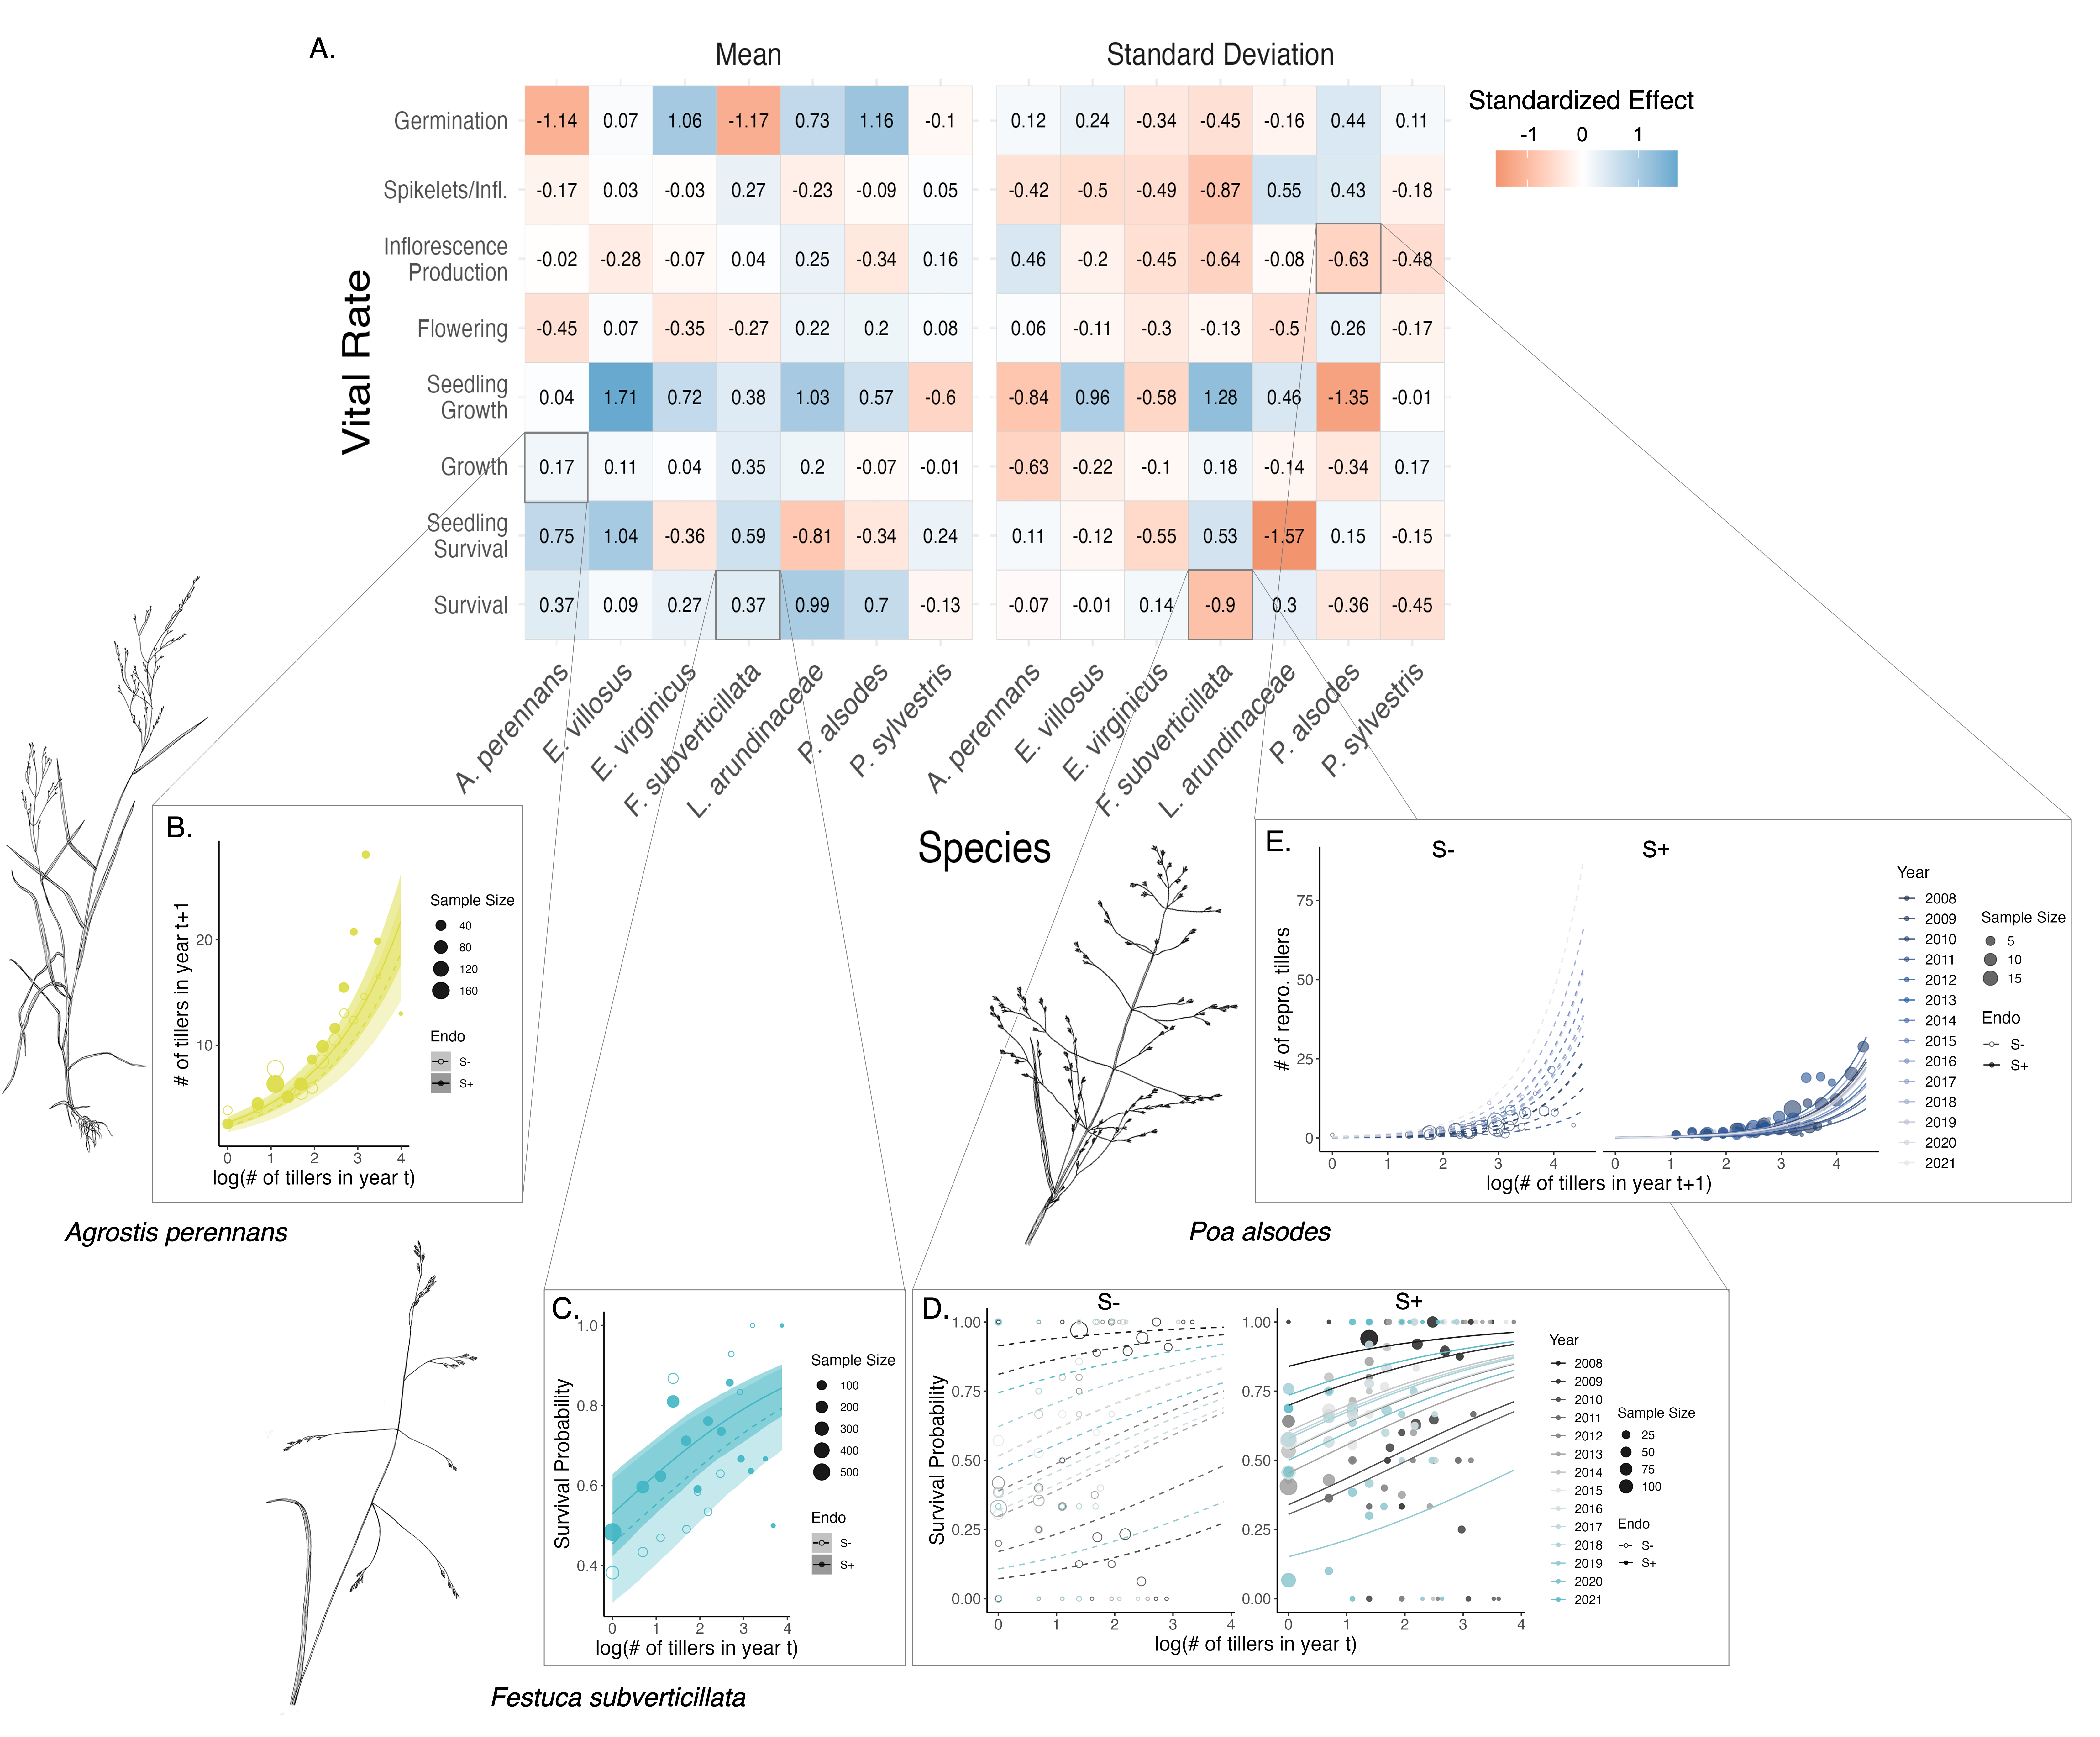
\includegraphics[width=\linewidth]{StochDemo_fig1_thesis.png}
	\caption{Endophyte symbiosis altered host vital rates.(A) Shading represents the posterior mean standardized effect size (Cohen's D) of endophyte symbiosis on mean or standard deviation of host vital rates (blue indicates that symbiosis increased the mean or standard deviation and red indicates a reduction). Endophytes' diverse vital rate effects include increased (B) mean growth of \emph{A. perennans} and (C) mean survival probability of \emph{F. subverticillata}. Endophyte presence also reduced inter-annual variance in (D) the survival of \emph{F. subverticillata} and (E) the fertility of \emph{P. alsodes}. Organism silhouettes modified from "Festuca subverticillata" by Cindy Roch\'e and "Agrostis hyemalis" and "Poa alsodes" by Sandy Long \copyright Utah State University.}
\end{figure*}

\begin{figure*}
	\centering
	\includegraphics[width =\linewidth]{StochDemo_fig2.png}
	\caption{Mean and variance-buffering effects on fitness. Black circles indicate the average effect of endophytes along with 500 posterior draws (smaller colored circles) on the (A) mean and (B) coefficient of variation in $\lambda$ for each host species as well as a cross species mean. (C) For all hosts, endophytes either reduce variance, increase the mean, or both, and consequently when considering stochastic environments, the interactions are always at least potentially mutualistic.}
\end{figure*}

\begin{figure*}
	\centering
	\includegraphics[width=.8\linewidth]{StochDemo_fig3.png}
	\caption{Host species with faster life history traits experience stronger effects of symbiont-mediated variance buffering. Regressions between life history traits describing the fast-slow life history continuum ((A) 99th percentile maximum age observed during long term censuses in years; (B) Seed size) and the effect of endophyte symbiosis on the coefficent of variation in population growth rate ($\lambda$). Each panel shows the fitted mean relationship (line) along with the 95\% credible interval.}
\end{figure*}

\begin{figure*}
	\centering
	\includegraphics[width=.8\linewidth]{StochDemo_fig4.png}
	\caption{Cross-species average endophyte contributions to stochastic growth rates under observed and elevated variance. Endophyte symbiosis contributes to the total effect of mutualism on $\lambda_{S}$ through benefits to mean growth rates and through variance buffering as well as the interaction between mean and variance effects. Shapes indicate the posterior mean of each contribution averaged across the seven focal symbiota, along with bars for the 50, 75 and 95\% credible intervals.  The full effect of the symbiosis (circles) becomes more mutualistic under scenarios of increased variance (represented by color shading). Relative to the ambient scenario sampling transition matrices for all 13 transition years during the study period, simulations increased variance by sampling the most extreme six or two years years, leading to increased contributions from variance buffering effects (triangles) and a constant contribution from mean effects (squares).}
\end{figure*}


\end{document}
